\documentclass[lasers.tex]{subfiles}

\begin{document}
\part{Quantum Information and Computing}
\chapter{}
\section{What is a quantum computer?}
It's like a classical computer, but we replace 'bits' (0s and 1s) with \emph{qubits.}
But what is a qubit?
A qubit is a 2-level quantum system, with the quantum levels referred to $|0\rangle$ and $|1\rangle$.

Examples of 2-level systems:
\begin{itemize}
    \item Spin-$\frac12$ particle: 2 states are spin 'up' and spin 'down'.
    \item Photon: 2 polarisations, e.g. vertical and horizontal or left-circular and right-circular.
    \item Atoms, ions, molecules with many energy levels and we can select 2 as our qubit states. 
    \item 'Artifical atoms' in solid state, e.g. quantum dots in semiconductors or LC resonator in a superconductor. 
\end{itemize}

List five physical implementations of qubits and their problems:
\begin{itemize}
    \item Two energy levels in an atom trapped by an optical tweezer - difficult to localise. 
    \item Two energy levels in an ion trapped using electrodes - it's only in one dimension (scaling problem). 
    \item Two energy levels of an impurity ion (spin) in a semi-conductor (e.g. phosphorous in Si) - interacts with surroundings, i.e. Silicon.
    \item Two energy levels of an LC circuit in a superconductor - very bulky and needs $10mK$ cryostat. 
    \item Two polarisation modes of a photon - photons don't interact. 
\end{itemize}

\chapter{}
\section{DiVincenzo Criteria}
The DiVincenzo criteria are often used to frame discussions about the advantages and disadvantages of different quantum computing platforms. 
The five criteria are:
\begin{enumerate}
    \item Initialisation (\textbf{state preparation}) - typically means the ability to prepare identical qubits through cooling and address each qubit independently (localisation).
    \item A universal set of quantum \textbf{gates} - single- and two-qubit gates at minimum. 
    \item Measurement (\textbf{read out}) of $|0\rangle$ or $|1\rangle$.
    \item Low \textbf{decoherence} - qubits isolated from environment (external world).
    \item \textbf{Scalability} - the ability to scale up to say 100 or 1000 or more qubits.
\end{enumerate}

\section{Why Quantum Computing?}
\begin{enumerate}
    \item Moore's law - as transistor size is reduced, we approach atomic dimensions.  
    \item Energy efficiency - replace dissipative classical gates with reversible quantum gates.
    \item Quantum 'advantage' - quantum computers can store more information and compute (certain problems) much faster.
\end{enumerate}
A classical bit has states 0 and 1: N bits have $2N$ states; a qubit has states $0\rangle$ and $|0\rangle$: N qubits have $2^N$ states, i.e. exponential scaling. 
To see why, we need the \textbf{Qubit State Vector}.
\begin{align}
    |\psi\rangle = a|0\rangle + b|1\rangle,
\end{align}
where $a$ and $b$ are complex coefficients that may be time-dependent which obey the normalisation criterion. 

Now we want a 2 qubit state vector, where our two qubits are A and B, as a normalised product state:
\begin{align}
    |\Psi\rangle_{AB} &= (a|0\rangle_A + b|1\rangle_A)\otimes(c|0\rangle_B+d|1\rangle_B), \\
                      &= ac|00\rangle + ad|01\rangle + bc|10\rangle + bd|11\rangle.
\end{align}
In addition to product, we can have \textbf{entangled states} that are not factorisable into products.

What about 3 qubits, $A,B,C$?
\begin{align}
    |\Psi\rangle_{ABC} &= c_{000}|000\rangle + c_{001}|001\rangle + c_{010}|010\rangle + c_{011}|011\rangle + c_{100}|100\rangle + c_{101}|101\rangle + c_{110}|110\rangle + c_{111}|111\rangle,
\end{align}
which is $2^3=8$ states. 
For 4 qubits, we would have $2^4=16$ states; for $N$ qubits, $2^N$ states. 
For 40 qubits, $2^{40}\approx10^{12}$; for 100 qubits, $2^{100}\approx10^{30}$.

\chapter{Two-level quantum mechanics}
Can think of the state vector similar to spin:
\begin{align}
    |\psi\rangle &= a|0\rangle + b|1\rangle = a|\uparrow\rangle + b|\downarrow\rangle = \begin{pmatrix} a \\ b\end{pmatrix}.
\end{align}
How does the time-dependence appear?
$0\rangle$ and $|1\rangle$ are solutions of a Schrodinger equation,
\begin{align}
    i\hbar\dpt|\alpha\rangle &= H_0|\alpha\rangle,
\end{align}
with energies $E_0$ and $E_1$:
\begin{align}
    i\hbar\dpt|0\rangle &= E_0|0\rangle,\; i\hbar\dpt|1\rangle = E_1|1\rangle, \\
    |\psi(t=0)\rangle &= a(0)|0\rangle \implies a(t) = a(0)e^{-iE_0t/\hbar},\\
    |\psi\rangle &= ae^{-iE_0t/\hbar}|0\rangle + be^{-iE_1t/\hbar}|1\rangle, \\
                 &= e^{-E_0t/\hbar}\left(a|0\rangle + be^{-i\om_0 t}|1\rangle\right).
\end{align}
$\om_0$ is the angular resonant frequency of the qubit, $\om_0=(E_1-E_0)/\hbar$.
We define
\begin{align}
    G &\equiv e^{-iE_0t/\hbar} \text{ - global phase}, & R &\equiv e^{-i\om_0t} \text{ - relative phase}.
\end{align}
\begin{align}
    |a|^2 &+ |b|^2 = 1 \\
    |\psi\rangle &= a|0\rangle + be^{i\phi}|1\rangle,
\end{align}
So only have two free parameters in the ratio $\frac{a}{b}$ and the phase $\phi$.
\begin{align}
    |\psi\rangle &= \begin{pmatrix}\cos\frac{\theta}{2} \\ e^{i\phi}\sin\frac{\theta}{2}\end{pmatrix} = \begin{pmatrix} a \\ be^{i\phi}\end{pmatrix} 
\end{align}
$\tan\frac{\theta}{2} = \frac{b}{a}$ and $\theta$ and $\phi$ are angles (from $z$ down and $x$ round respectively as spherical coordinates. 
So we can talk about our state vector as a Bloch vector, with all possible states of the qubit are points on the Bloch sphere.

\section{Single-qubit gates}
All single qubits are rotations on the Bloch sphere. 
These rotations are described by unitary operator, e.g. $U$,
\begin{align}
    |\psi_f\rangle &= U|\psi_i\rangle,
\end{align}
where $U$ is a $2\times2$ matrix. 
We can write $U$ as a sum of Pauli spin matrices (and the identity matrix),
\begin{align}
    \hat{\sigma}_x &= \begin{pmatrix}0&1\\1&0\end{pmatrix}, & \hat{\sigma}_y &= \begin{pmatrix}0&-i\\i&0\end{pmatrix}, & \hat{\sigma}_z &= \begin{pmatrix}1&0\\0&-1\end{pmatrix}, & \hat{\sigma}_0 &= \begin{pmatrix}1&0\\0&1\end{pmatrix}.
\end{align}

\begin{example}[Density operator]
    The density operator is defined as:
    \begin{align}
        \hat{\rho} &= |\psi\rangle\langle\psi|.
    \end{align}
    We will write this in the form of the Pauli matrices and identity, then as a single matrix:
    \begin{align}
        \hat{\rho} &= \frac12\left(\hat{\sigma}_0 + u\hat{\sigma}_x + v\hat{\sigma}_y + w\hat{\sigma}_z\right) \\
                   &= \frac12\begin{pmatrix} 1+w & u-iv \\ u+iv & 1-w\end{pmatrix}.
    \end{align}
    $u,v,w$ are the expectation values of $\hat{\sigma}_x,\hat{\sigma}_y,\hat{\sigma}_z$ for the state $|\psi\rangle$.
\end{example}

\begin{example}[Short Question \#7]
    Let's take a particular state,
    \begin{align}
        |\psi\rangle &= \frac{1}{\sqrt{2}}\left(|0\rangle+e^{i\phi}|1\rangle\right).
    \end{align}
    What is the value of $\theta$?
    \begin{align}
        \cos\frac{\theta}{2} &= \sin\frac{\theta}{2} = \frac{1}{\sqrt{2}} \implies \frac{\theta}{2} = \frac{\pi}{4} \implies \theta = \frac{\pi}{2}.
    \end{align}
    Bloch vector is in equatorial plane. 
    Now calculate expectation values of $\hat{\sigma}_i$:
    \begin{align}
        \langle\psi|\hat{\sigma}_x|\psi\rangle &= \frac{1}{\sqrt{2}}\begin{pmatrix} 1 & e^{-i\phi}\end{pmatrix}\begin{pmatrix}0 & 1 \\ 1 & 0 \end{pmatrix}\frac{1}{\sqrt{2}}\begin{pmatrix}1 \\ e^{i\phi}\end{pmatrix} \\
                                               &= \frac12\left(e^{i\phi}+e^{-i\phi}\right) = \cos\phi.
    \end{align}
    $\phi=0\implies u=+1, \phi=\pi \implies u=-1$.
    \begin{align}
        \langle\psi|\hat{\sigma}_y|\psi\rangle &= \frac12\begin{pmatrix}1 & e^{-i\phi}\end{pmatrix}\begin{pmatrix}0 & -i \\ i & 0\end{pmatrix}\begin{pmatrix} 1 \\ e^{i\phi}\end{pmatrix} \\
                                               &= \frac{1}{2i}\left(e^{i\phi}+e^{-i\phi}\right) = \sin\phi. \\
        \langle\psi|\hat{\sigma}_z|\psi\rangle &= \frac12\begin{pmatrix} 1 & e^{-i\phi}\end{pmatrix}\begin{pmatrix}1 & 0 \\ 0 & -1\end{pmatrix}\begin{pmatrix}1 \\ e^{i\phi}\end{pmatrix} \\
                                               &= \frac12\left(1-1\right) = 0.
    \end{align}
    So the Bloch vector is in equatorial plain as thought. 
\end{example}

\chapter{}
\begin{itemize}
    \item Any qubit can be represented by a point on the Bloch sphere. 
    \item We have two parameters: the polar angle, $\theta$; and the azimuthal angle, $\phi$.
    \item The qubit state vector is defined as
        \begin{align}
            |\psi\rangle = \begin{pmatrix} \cos\frac{\theta}{2}\\ e^{i\phi}\sin\frac{\theta}{2}\end{pmatrix} = \begin{pmatrix} a \\ b\end{pmatrix}.
        \end{align}
\end{itemize}
In Cartesian coordinates, the qubit state is given by the Bloch vector $\vec{b}=(u,v,w)$, with $\sqrt{u^2+v^2+w^2}=1$.
This Cartesian description allows for
    \begin{align}
        \sqrt{u^2+v^2+w^2} &< 1,
    \end{align}
i.e. point inside the sphere.
In the real world, we have decoherence where the effect is to shorten the Bloch vector.
We have two types of states:
\begin{itemize}
    \item Pure states: $\sqrt{u^2+v^2+w^2}=1$, on the Bloch sphere, represented by the wavefunction $|\psi\rangle$.
    \item Mixed states: $\sqrt{u^2+v^2+w^2} < 1$, inside the Bloch sphere.
\end{itemize}
We cannot describe mixed states by a wavefunction, so we introduce the density matrix.

\section{Density matrix for a pure state of a qubit}
We define the density matrix as:
\begin{align}
    \rho &= |\psi\rangle\langle\psi| = \begin{pmatrix} \cos\frac{\theta}{2} \\ e^{i\phi}\sin\frac{\theta}{2}\end{pmatrix}\begin{pmatrix} \cos\frac{\theta}{2} & e^{-i\phi}\sin\frac{\theta}{2}\end{pmatrix}  \\
                                    &= \begin{pmatrix} \cos^2\frac{\theta}{2} & e^{-i\phi}\sin\frac{\theta}{2}\cos\frac{\theta}{2} \\ e^{i\phi}\sin\frac{\theta}{2}\cos\frac{\theta}{2} & \sin^2\frac{\theta}{2}\end{pmatrix} = \frac12 \begin{pmatrix} 1+\cos\theta & e^{-i\phi}\sin\theta \\ e^{i\phi}\sin\theta & 1-\cos\theta\end{pmatrix} \\
                                    &= \frac12 \begin{pmatrix} 1+\cos\theta & \sin\theta\cos\phi - i\sin\theta\sin\phi \\ \sin\theta\cos\phi + i\sin\theta\sin\phi & 1-\cos\theta\end{pmatrix} \\
    \rho &= \frac12\begin{pmatrix} 1+w & u-iv \\ u+iv & 1-w\end{pmatrix} = \frac12\left(\hat{\sigma}_0 + u\hat{\sigma}_x + v\hat{\sigma}_y + w\hat{\sigma}_z\right).
\end{align}
What is the expectation value of $\rho$ for our wavefunction?
If we have a normalised wavefunction, $\langle\psi|\rho|\psi\rangle = \langle\psi|\psi\rangle\langle\psi|\psi\rangle = 1$.
\begin{align}
    \langle\psi|\rho|\psi\rangle &= \frac12\left(\langle\psi|\sigma_0|\psi\rangle + u\langle\psi|\sigma_x|\psi\rangle + \cdots\right) \\
                                 &= \frac12\left(1 + u^2 + v^2 + w^2\right) = 1
\end{align}
For mixed states, $\sqrt{u^2+v^2+w^2}<1$, so this will no longer be the case. 
We will explore that properly later. 

\section{Qubit Rotations}
All unitary operations (that conserve the norm $\langle\psi|\psi\rangle$) can be described as rotations of the Bloch vector. 
A general rotation by an angle $\Theta$ about a unit vector $\vec{n}=(n_x,n_y,n_z)$.
We define the Rotation operator, 
\begin{align}
    \hat{R} &= \exp\left(-i\frac12\hat{\vec{\sigma}}\cdot\vec{n}\Theta\right) \\
            &= \hat{\sigma}_0\cos\frac{\Theta}{2} - i\hat{\vec{\sigma}}\cdot\vec{n}\sin\frac{\Theta}{2} \\
            &= \begin{pmatrix} \cos\frac{\Theta}{2}-in_z\sin\frac{\Theta}{2} & \left(-in_x-ny\right)\sin\frac{\Theta}{2} \\ \left(-in_x+n_y\right)\sin\frac{\Theta}{2} & \cos\frac{\Theta}{2}+in_z\sin\frac{\Theta}{2}  \end{pmatrix}
\end{align}

\chapter{}
How do we implement rotation on the Bloch sphere?
We need to drive the qubit with a resonant (or near-resonant) EM field. 
\begin{figure}[H]
    \centering
    \begin{tikzpicture}
        \draw[-Latex] (0,1) node[anchor=north] {EM field} sin (0.5,2) cos (1,1) sin (1.5,0) cos (2,1) sin (2.5,2) cos (3,1) sin (3.5,0) cos (4,1) sin (4.5,2) cos (5.25,1.35) sin (6.5,0.6);
        \draw (8,1) circle (30pt);
        \draw (7.3,0.4) node[anchor=east,xshift=-5pt] {$E_0$} -- (8.7,0.4) node[anchor=west,xshift=5pt] {$|1\rangle$};
        \draw (7.3,1.6) node[anchor=east,xshift=-5pt] {$E_1$} -- (8.7,1.6) node[anchor=west,xshift=5pt] {$|0\rangle$};
        \draw[-Latex] (8.4,0.4) -- (8.4,1.6) node[anchor=east,midway] {$\hbar\om_0$};
    \end{tikzpicture}
\end{figure}
The qubit is like an oscillator we can drive. 
EM field:
\begin{align}
    \mathcal{E} &= \mathcal{E}_0\cos(\phi_L-\om t),
\end{align}
where $\phi_L$ is the laser phase.
We could include any phase offset. 
We assume the qubit is at $\vr=0$, and $\phi=0$ at $t=0$, so $\phi_L=\vec{k}\cdot\vr$.
This then depends on the relative position of the qubit and field. 
Note that since there is always some $\delta r$ uncertainty in position of the qubit, this gives rise to a range of phase $\phi_L$ which can influence the qubit behaviour, e.g. phonons are solid vibrating all the time $\to$ phase is changing. 
Hence inside the sphere for the qubit and not on the sphere. 
We can try to reduce this by lowering temperatures. 
Other notation:
\begin{align}
    \Delta &= \om-\om_0,
\end{align}
where $\om_0$ is the qubit frequency, $\om$ the field frequency, and $\Delta$ is defined as the qubit-field detuning. 
If the qubit is subject to an external field, the coefficients $a$ and $b$ may become functions of time, and we should write the qubit state vector in the form
\begin{align}
    |\psi(t)\rangle &= a(t)|0\rangle e^{-iE_0t/\hbar} + b(t)|1\rangle e^{-iE_1t/\hbar}.
\end{align}
The time dependence of the coefficients $a$ and $b$ depends on the interaction between the qubit and the EM field. 
We can use the Schrodinger equation:
\begin{align}
    i\hbar\dpt|\psi\rangle &= (\Ham_0+\Ham')|\psi\rangle.
\end{align}
Previously we just had $\Ham_0$ which describes the qubit, but now we add $\Ham'$ which is the perturbation due to the EM field.
Typically, this interaction is of the form 
\begin{align}
    \Ham' &= -\hat{\vec{d}}\cdot\vec{\mathcal{E}},
          &= -d\mathcal{E}_0\cos(\phi_L-\om t),
\end{align}
where $\vec{d}=-e\hat{\vr}$ is the electric dipole operator.
and we can also define the Rabi frequency in Hz as
\begin{align}
    \Omega &= -\frac{d\mathcal{E}_0}{\hbar}, \\
    \Ham' &= \hbar\Omega\cos(\phi_L-\om t).
\end{align}
The Rabi frequency is a measure of the coupling between the field and the qubit. 
If the field is put on and left on, then the state will oscillate between $|0\rangle$ and $|1\rangle$ at the Rabi frequency. 
Subbing the perturbation, we get two equations for $a$ and $b$:
\begin{align}
    i\dot{a}(t) &= \frac12\Omega e^{-i\phi_L}e^{i\Delta\cdot t}b, & i\dot{b}(t) &= \frac12\Omega e^{i\phi_L}e^{-i\Delta\cdot t}a.
\end{align}
These equations have an explicit time dependence.
To deal with this, we can go into a rotating frame using a substitution:
\begin{align}
    \tilde{a} &= ae^{-it\cdot\Delta/2}, & \tilde{b} &= be^{it\cdot\Delta/2}.
\end{align}
This is so that we spin at the same frequency as the qubit and since we are interested in the relative phase of the field and qubit, this makes sense. 
The Schrodinger equation for the interaction between a qubit and an oscillatory EM field is
\begin{align}
    i\hbar\dpt|\psi\rangle &= \Ham_{int}|\psi\rangle,
\end{align}
where for the vector for of the state vector, the \textbf{interaction Hamiltonian} is a $2\times2$ matrix:
\begin{align}
    \Ham_{int} &= \frac{\hbar}{2}\begin{pmatrix} \Delta & \Omega e^{-i\phi_L} \\ \Omega e^{i\phi_L} & -\Delta\end{pmatrix}, \\
    i\hbar\dpt \begin{pmatrix}\tilde{a}\\ \tilde{b}\end{pmatrix} &= \frac{\hbar}{2}\begin{pmatrix}\Delta & \Omega e^{-i\phi_L} \\ \Omega e^{i\phi_L} & -\Delta\end{pmatrix}\begin{pmatrix}\tilde{a}\\ \tilde{b}\end{pmatrix}.
\end{align}
We can also write $\Ham_{int}$ in terms of the spin matrices. 
Note that we have the detuning on the diagonals (like $\hat{\sigma}_z$) and to get the exponential, we need $\cos$ and $\sin$ terms:
\begin{align}
    \Ham_{int} &= \frac{\hbar}{2}\left[\Delta\hat{\sigma}_z + \Omega\left(\cos\phi_L\hat{\sigma}_x + \sin\phi_L\hat{\sigma}_y\right)\right],
\end{align}
where $\hat{\sigma}_y$ contains the imaginary values necessary for the exponents. 
Consider zero detuning, i.e. $\Delta=0,\om_0=\om,$ and $\phi_L=0$:
\begin{align}
    i\dot{a} &= \frac12 \Omega b, & i\dot{b} &= \frac12\Omega a.
\end{align}
Taking time derivatives again:
\begin{align}
    i\ddot{a} &= \frac12\Omega\dot{b} = -\frac{i}{4}\Omega a \implies \ddot{a} = -\frac14\Omega^2 a.
\end{align}
For $a(0)=1,b(0)=0$, $a=\cos\left(\frac{\Omega t}{2}\right)$.
Getting probabilities:
\begin{align}
    P_{|0\rangle} &= |a|^2 = \cos^2\left(\frac{\Omega t}{2}\right) = \frac12(1+\cos\Omega t), \\
    P_{|1\rangle} &= |b|^2 = \sin^2\left(\frac{\Omega t}{2}\right) = \frac12(1-\cos\Omega t),
\end{align}
\begin{figure}[H]
    \centering
    \begin{tikzpicture}
        \draw[-Latex] (0,0) -- (6,0) node[anchor=north] {t};
        \draw[-Latex] (0,0) -- (0,2.8) node[anchor=east] {P};
        \draw[purple] (0,2.5) node[anchor=east,black] {1} cos (1,1.25) sin (2,0) node[anchor=north,black] {$\frac{\pi}{\Omega}$} cos (3,1.25) sin (4,2.5) cos (5,1.25) sin (6,0) node[anchor=south west] {$P_{|0\rangle}$};
        \draw[cyan] (0,0) node[anchor=east,black] {0} cos (1,1.25) sin (2,2.5) cos (3,1.25) sin (4,0) node[anchor=north,black] {$\frac{2\pi}{\Omega}$} cos (5,1.25) sin (6,2.5) node[anchor=west] {$P_{|1\rangle}$};
    \end{tikzpicture}
\end{figure}
$\theta=\frac{\Omega t}{2}$ is the rotation angle. 
The effect of the resonant EM field is to drive the qubit from $|0\rangle\to|1\rangle$ and back at $\Omega$ frequency. 

The qubit follows a line of longitude. 
$\phi_L$ determines the direction in the $xy$ plane about which we rotate, i.e. can change which longitude line we travel around. 
Derive rotation matrix $\hat{R}$ from the interaction Hamiltonian:
\begin{align}
    |\psi(t)\rangle &= e^{-i\Ham_{int}t/\hbar}|\psi(0)\rangle = \hat{R}|\psi(0)\rangle.
\end{align}
To find the rotation matrix, we rewrite the interaction in the form:
\begin{align}
    \hat{R} &= e^{-i\Ham_{int}t/\hbar} = e^{-(i/2)\hat{\sigma}\cdot\hat{\vec{n}}\Theta},\quad \Theta = t\sqrt{\Omega^2+\Delta^2}.
\end{align}
We had defined $\Ham_{int}$ as 
\begin{align}
    \Ham_{int} &= \frac{\hbar}{2}\left[\Delta\hat{\sigma}_z + \Omega\left(\cos\phi_L\hat{\sigma_x}+\sin\phi_L\hat{\sigma}_y\right)\right],
\end{align}
so using this in $\hat{R}$ above, we can determine $\hat{\vec{n}}$ to be
\begin{align}
    \hat{\vec{n}} &= \frac{1}{\Theta}\begin{pmatrix} \Omega\cos\phi_L & \Omega\sin\phi_L & \Delta\end{pmatrix}.
\end{align}

\chapter{}
From normalisation we define $\Theta=t\sqrt{\Omega^2+\Delta^2}$, with the quantity in brackets known as the \emph{effective Rabi frequency.}
Substituting the unit vector $\hat{\vec{n}}$ above into the rotation matrix:
\begin{align}
    \hat{R} &= \begin{pmatrix} \cos\frac{\theta}{2}-in_z\sin\frac{\theta}{2} & (-in_x-n_y)\sin\frac{\theta}{2} \\ (-in_x+n+y)\sin\frac{\theta}{2} & \cos\frac{\theta}{2}+in_z\sin\frac{\theta}{2}\end{pmatrix} \\
            &= \begin{pmatrix} \cos\frac{\theta}{2}-i\frac{\Delta}{\Theta}\sin\frac{\theta}{2} & -i\frac{\Omega}{\Theta}e^{i\phi_L}\sin\frac{\theta}{2} \\ -i\frac{\Omega}{\Theta}e^{-i\phi_L}\sin\frac{\theta}{2} & \cos\frac{\theta}{2}+i\frac{\Delta}{\Theta}\sin\frac{\theta}{2}\end{pmatrix}.
\end{align}
This is known as the \textbf{Rabi solution.}
We consider the first of 3 special cases:\\
Case 1: $\Delta=0$, i.e. on resonance. The Rabi solution reduces to
\begin{align}
    \hat{R} &= \begin{pmatrix} \cos\frac{\Omega t}{2} & -ie^{i\phi_L}\sin\frac{\Omega t}{2} \\ -ie^{-i\phi_L}\sin\frac{\Omega t}{2} & \cos\frac{\Omega t}{2}\end{pmatrix},
\end{align}
which corresponds to a rotation about a vector in the equatorial plane in the Bloch sphere.
For $\Delta=0$, we often use notation $\hat{R}(\theta,\phi_L)$ where $\theta=\frac{\Omega t}{2}$ is the rotation angle and $\phi_L$ determines the direction in the $xy$ plane about which we rotate. 
For an atom initially in state $|0\rangle$, i.e.
\begin{align}
    |\psi(0)\rangle &= \begin{pmatrix}1\\ 0\end{pmatrix} = |0\rangle,
\end{align}
and an interaction of duration $t$, the Rabi solution gives
\begin{align}
    |\psi(t)\rangle &= \hat{R}|\psi(0)\rangle = \begin{pmatrix} \cos\frac{\Omega t}{2} \\ -ie^{-i\phi_L}\sin\frac{\Omega t}{2} \end{pmatrix} = \begin{pmatrix} a(t) \\ b(t)\end{pmatrix}, \\
    a(t) &= \cos\frac{\Omega t}{2}, \qquad b(t) = -ie^{-i\phi_L}\sin\frac{\Omega t}{2},
\end{align}
and we get the populations in states $|0\rangle,|1\rangle$ from
\begin{align}
    P_{|0\rangle} &= |a(t)|^2 = \cos^2\frac{\Omega t}{2},\\
    P_{|1\rangle} &= |b(t)|^2 = \sin^2\frac{\Omega t}{2},
\end{align}
which are the \textbf{Rabi oscillations.}
The population oscillates between the two states at the Rabi frequency, $\Omega$.
The Rabi frequency is proportional to the field amplitude, i.e. the square root of the field intensity. 
\begin{figure}[H]
    \centering
    \begin{tikzpicture}
        \draw[-Latex] (0,0) -- (6,0) node[anchor=north] {t};
        \draw[-Latex] (0,0) -- (0,2.8) node[anchor=east] {P};
        \draw[purple] (0,2.5) node[anchor=east,black] {1} cos (1,1.25) sin (2,0) node[anchor=north,black] {$\frac{\pi}{\Omega}$} cos (3,1.25) sin (4,2.5) cos (5,1.25) sin (6,0) node[anchor=south west] {$P_{|0\rangle}$};
        \draw[cyan] (0,0) node[anchor=east,black] {0} cos (1,1.25) sin (2,2.5) cos (3,1.25) sin (4,0) node[anchor=north,black] {$\frac{2\pi}{\Omega}$} cos (5,1.25) sin (6,2.5) node[anchor=west] {$P_{|1\rangle}$};
        \draw[dashed] (1,0) node[anchor=north] {$\frac{\pi}{2\Omega}$} -- (1,1.25);
    \end{tikzpicture}
\end{figure}
Another interesting case is when there is no interaction ($\Omega=0$) but the field and the qubit have a different frequency $\Delta\neq0$, i.e. \emph{free evolution rotations}.
In this case, the rotation matrix is 
\begin{align}
    \hat{R} &= \begin{pmatrix} \exp\left(-i\frac{\Delta t}{2}\right) & 0 \\ 0 & \exp\left(i\frac{\Delta t}{2}\right)\end{pmatrix},
\end{align}
which corresponds to a rotation about the z-axis in the Bloch sphere. 
We use this matrix to describe the free evolution in a \emph{Ramsey interferometer}.

\section{Single Qubit Rotations}
The Rabi solution describes how a near-resonance EM field may be used to drive the qubit from any initial state to any final state. 
Refer to this operation as a \textbf{single-qubit rotation} or \textbf{single-qubit gate.}
Three useful interactions come from the times you pulse, e.g. as above the $\frac{\pi}{2}$-, $\pi$-, and $2\pi$-pulse.
For all except the \textbf{Hadamard gate}, we use resonant driving $\Delta=0$.
\begin{itemize}
    \item $\frac{\pi}{2}$-pulse (particularly useful):\\
        For a $\frac{\pi}{2}$ pulse, we choose the EM field intensity and the pulse duration such that $\Omega t=\frac{\pi}{2}$. 
        This corresponds to a rotation of $90^\circ$ on the Bloch sphere which could take us from pole to equator, i.e. a qubit initially in $|0\rangle$ or $|1\rangle$ is excited $\to$ an equal superposition on the equator (or start on the equator and rotate to a pole).
        Substituting $\Omega t=\frac{\pi}{2}$ in the Rabi solution, we obtain
        \begin{align}
            |\psi(t_{\pi/2})\rangle &= \frac{1}{\sqrt{2}} \begin{pmatrix} 1 & -ie^{i\phi_L} \\ -ie^{-i\phi_L} & 1\end{pmatrix}|\psi(0)\rangle.
        \end{align}
        To simplify the matrix, we can choose a particular laser phase, e.g. $\phi_L=\frac{\pi}{2}$, so:
        \begin{align}
            \hat{R}(\theta,\phi_L) &= \hat{R}\left(\frac{\pi}{2},\frac{\pi}{2}\right) = \frac{1}{\sqrt{2}}\begin{pmatrix}1 & 1 \\ -1 & 1\end{pmatrix},
        \end{align}
        and acting on our initial state $|\psi(0)\rangle=|0\rangle$,
        \begin{align}
            |\psi(t_{\pi/2})\rangle &= \hat{R}\left(\frac{\pi}{2},\frac{\pi}{2}\right)|\psi(0)\rangle \\
                                    &= \frac{1}{\sqrt{2}}\begin{pmatrix}1&1\\-1&1\end{pmatrix}\begin{pmatrix}1\\0\end{pmatrix} = \frac{1}{\sqrt{2}}\begin{pmatrix}1\\-1\end{pmatrix} \\
                                    &= \frac{1}{\sqrt{2}}\left(|0\rangle-|1\rangle\right),
        \end{align}
        which is a superposition between $|0\rangle$ and $|1\rangle$. 
        This corresponds to a rotation around the $y$ axis, ending up in the $-x$ direction, i.e. the expectation value $\langle\hat{\sigma}\rangle=-1$.
        If we apply an arbitrary phase $\phi_L$ to $|1\rangle$, we find
        \begin{align}
            |1\rangle &\to \frac{1}{\sqrt{2}}\left(-ie^{i\phi_L}|0\rangle+|1\rangle\right).
        \end{align}
        For $\phi_L=0$, we would rotate around the $x$ axis and end up along $y$. 
        So the laser phase sets the vector in the $xy$ plane that we rotate around. 
        If we had started with a superposition, e.g. in Eq (6.14), it carries on to the $|1\rangle$ state if we apply the same $\hat{R}\left(\frac{\pi}{2},\frac{\pi}{2}\right)$:
        \begin{align}
            \hat{R}\left(\frac{\pi}{2},\frac{\pi}{2}\right)\frac{1}{\sqrt{2}}\begin{pmatrix}1 \\ -1\end{pmatrix} &= \frac12\begin{pmatrix}1&1\\-1&1\end{pmatrix}\begin{pmatrix}1\\-1\end{pmatrix} = - \begin{pmatrix} 0 \\ 1\end{pmatrix}.
        \end{align}
        So 2 $\frac{\pi}{2}$ pulses are equivalent to a $\pi$-pulse and takes us from $|0\rangle\to|1\rangle$.
        We shouldn't be concerned about the '$-1$' as when we take the modulus this global phase disappears. 
    \item $\pi$-pulse: For $\Omega t_\pi = \pi$,
        \begin{align}
            |\psi(t_\pi)\rangle &= \begin{pmatrix} 0 & -ie^{i\phi_L}\\ -ie^{-i\phi_L} & 0 \end{pmatrix}|\psi(0)\rangle,\\
            |0\rangle &\to -ie^{-i\phi_L}|1\rangle,\qquad |1\rangle \to -ie^{i\phi_L}|0\rangle.
        \end{align}
        For $\phi_L=0$ and $\phi_L=\frac{\pi}{2}$ respectively, the rotation matrix is
        \begin{align}
            \hat{R}\left(\pi,0\right) &= \begin{pmatrix}0&-i\\-i&0\end{pmatrix}; & \hat{R}\left(\pi,\frac{\pi}{2}\right) &= \frac{1}{\sqrt{2}}\begin{pmatrix}0&1\\-1&0\end{pmatrix}.
        \end{align}
        Except for the sign change, this is equivalent to a '\emph{bit-flip}' or \emph{NOT gate}.
    \item $2\pi$-pulse:
        For $\Omega t_{2\pi}=2\pi$, we have
        \begin{align}
            \hat{R}\left(2\pi,\phi_L\right) &= \begin{pmatrix}-1&0\\0&-1\end{pmatrix} = -\hat{\sigma}_0,
        \end{align}
        so it effectively just multiplies the entire wavefunction by $-1$, which is a global phase factor (and property of spin-$\frac12$ particles) that can be useful in gate operations.
        In the case of two qubits, if one of them picks up a $-1$, then it does become significant as they are entangled and we can now detect this. 
\end{itemize}

\section{Hadamard Gate}
The application of two successive $\frac{\pi}{2}$-pulses inverts the state. 
However, it is also useful to have a pulse that takes us into a superposition and back to the same state. 
This is a \textbf{Hadamard gate} or \textbf{Hadamard transform}.
The Hadamard operator is 
\begin{align}
    \Ham &= \frac{1}{\sqrt{2}}\begin{pmatrix}1&1\\1&-1\end{pmatrix},
\end{align}
and the application of two of these leave the state unchanged, i.e. $\Ham^2 = \hat{\sigma}_0$ (as long as nothing happens in-between applying them).
There are different ways to implement a Hadamard. 
One os to set $\Delta=\Omega$, in which case the Rabi solution becomes
\begin{align}
    \hat{R} &= \begin{pmatrix} \cos\frac{\Omega}{\sqrt{2}}t-\frac{i}{\sqrt{2}}\sin\frac{\Omega}{\sqrt{2}}t & -\frac{i}{\sqrt{2}}e^{i\phi_L}\sin\frac{\Omega}{\sqrt{2}}t \\  -\frac{i}{\sqrt{2}}e^{-i\phi_L}\sin\frac{\Omega}{\sqrt{2}}t & \cos\frac{\Omega}{\sqrt{2}}t+\frac{i}{\sqrt{2}}\sin\frac{\Omega}{\sqrt{2}}t \end{pmatrix},
\end{align}
and if we set $\frac{\Omega}{\sqrt{2}}t = \frac{\pi}{2}$ and $\phi_L=0$, we obtain
\begin{align}
    \hat{R} &= -\frac{i}{\sqrt{2}}\begin{pmatrix}1&1\\1&-1\end{pmatrix},
\end{align}
so $\hat{R}$ is the Hadamard up to some global factor which can be ignored. 
The Hadamard is a rotation around some $45^\circ$; applying twice brings us back to the start.

\chapter{}
\section{Ramsey Interferometry}
We have two $\frac{\pi}{2}$ pulses separated by time $t$ (or Hadamards):
\begin{figure}[H]
    \centering
    \begin{tikzpicture}
        %Nodes
        \node[roundnode] (maintopic) {$\frac{\pi}{2}$};
        \node[roundnode] (uppercircle) [above right=2em and 7em of maintopic] {$\frac{\phi}{2}$};
        \node[roundnode] (lowercircle) [below right=2em and 7em of maintopic] {$\frac{-\phi}{2}$};
        \node[roundnode] (output) [right=15em of maintopic] {$\frac{\pi}{2}$};
        \node (start) [left=1em of maintopic] {};
        \node (end) [right=1em of output] {};
        \node (ups) [above right=0.9em and 3.1em of maintopic] {};
        \node (ds) [below right=0.9em and 3.1em of maintopic] {};
        \node (upe) [above left=0.9em and 3em of output] {};
        \node (de) [below left=0.9em and 3em of output] {};

        %Lines
        \draw (start.east) -- (maintopic.west);
        \draw (output.east) -- (end.west);
        \draw (maintopic.east) cos (ups) sin (uppercircle.west);
        \draw (maintopic.east) cos (ds) sin (lowercircle.west);
        \draw (uppercircle.east) cos (upe) sin (output.west);
        \draw (lowercircle.east) cos (de) sin (output.west);
    \end{tikzpicture}
\end{figure}
We can also schematically represent paths in Hilbert space:
\begin{figure}[H]
    \centering
    \begin{tikzpicture}
        \draw (0,0) node[anchor=east] {$|\psi\rangle=$} -- (1,0);
        \draw (1,-0.25) rectangle (2.5,0.25) node[anchor=north east,xshift=-14pt] {H};
        \draw (2.5,0) -- (3.5,0);
        \draw (3.5,-0.25) rectangle (5,0.25) node[anchor=north east,xshift=-14pt] {H};
        \draw (6,0) -- (5,0);

        \draw (0,1) node[anchor=east] {$|\psi\rangle=$} -- (1,1);
        \draw (1,0.75) rectangle (2.5,1.25) node[anchor=north east,xshift=-14pt,yshift=2pt] {$\frac{\pi}{2}$};
        \draw (2.5,1) -- (3.5,1);
        \draw (3.5,0.75) rectangle (5,1.25) node[anchor=north east,xshift=-14pt,yshift=2pt] {$\frac{\pi}{2}$};
        \draw (6,1) -- (5,1);

        \draw (0,1.75) -- (1,1.75);
        \draw (1,1.75) -- (1,2.25) -- (2.5,2.25) node[anchor=north,midway,yshift=2pt] {$\frac{\pi}{2}$} -- (2.5,1.75) -- (3.5,1.75) -- (3.5,2.25) -- (5,2.25) node[anchor=north,midway,yshift=2pt] {$\frac{\pi}{2}$} -- (5,1.75) -- (6,1.75);
        \draw[Latex-Latex] (1.75,2.35) -- (4.25,2.35) node[anchor=south,midway] {$t$};
    \end{tikzpicture}
\end{figure}
There is a read-out of relative phase. 
This interval $t$ is often called the \emph{free evolution time,} but this could include an interaction. 
During this free evolution, the qubit Bloch vector rotates around the $z$-axis.
We can describe this precession using a rotation matrix:
\begin{align}
    \hat{R}_z(\phi) &= \begin{pmatrix} e^{i-\phi/2} & 0 \\ 0 & e^{-\phi/2} \end{pmatrix} = \begin{pmatrix} e^{-i\Delta t/2} & 0 \\ 0 & e^{i\Delta t/2} \end{pmatrix},
\end{align}
so we can say that the Bloch vector precesses around the $z$-axis at a rate given by the difference between the field and qubit evolution, $\Delta=\om-\om_0$.
The total rotation angle is $\phi=\Delta t$.

The complete Ramsey sequence is given by two $\frac{\pi}{2}$ pulses separated by free evolution. 
The $\frac{\pi}{2}$ pulse matrix is obtained from the Rabi solution for $\Delta = 0$.
\begin{align}
    \hat{R} &= \begin{pmatrix} \cos\frac{\theta}{2} & -ie^{i\phi_L}\sin\frac{\theta}{2} \\ -ie^{-i\phi_L}\sin\frac{\theta}{2} & \cos\frac{\theta}{2}\end{pmatrix},
\end{align}
where $\theta=\Omega t$.
We choose $\phi_L=\frac{\pi}{2}$:
\begin{align}
    \hat{R}\left(\frac{\pi}{2},\frac{\pi}{2}\right) &= \frac{1}{\sqrt{2}}\begin{pmatrix} 1 & 1 \\ -1 & 1\end{pmatrix} = \hat{R}_y\left(\frac{\pi}{2}\right).
\end{align}
Our complete sequence is given by $\hat{R}\left(\frac{\pi}{2}\right)\hat{R}\left(\phi\right)\hat{R}_y\left(\frac{\pi}{2}\right)$, where we write our sequence of rotations in reverse order. 
\begin{align}
    \hat{R}_y\left(\frac{\pi}{2}\right)\hat{R}(\phi)\hat{R}\left(\frac{\pi}{2}\right) &= \frac12 \begin{pmatrix} 1 & 1 \\ -1 & 1\end{pmatrix}\begin{pmatrix} e^{-i\phi/2} & 0 \\ 0 & e^{i\phi/2}\end{pmatrix} \begin{pmatrix} 1 & 1 \\ -1 & 1\end{pmatrix} \\
                                                                                      &= \frac12 \begin{pmatrix} 1 & 1 \\ -1 & 1\end{pmatrix} \begin{pmatrix} e^{-i\phi/2} & e^{-i\phi_2} \\ -e^{-\phi/2} & e^{i\phi/2}\end{pmatrix} \\
                                                                                      &= \begin{pmatrix} -i\sin\frac{\phi}{2} & \cos\frac{\phi}{2} \\ -\cos\frac{\phi}{2} & i\sin\frac{\phi}{2}\end{pmatrix}.
\end{align}
Initial Condition (at the North Pole):
\begin{align}
    |\psi\rangle &= |0\rangle = \begin{pmatrix} 1 \\ 0 \end{pmatrix} \\
    \hat{R}\left(\frac{\pi}{2}\right)\hat{R}_z(\phi)\hat{R}_y\left(\frac{\pi}{2}\right)|\psi\rangle &= \begin{pmatrix} -\sin\frac{\phi}{2} \\ -\cos\frac{\phi}{2}\end{pmatrix} 
\end{align}
Our output state has:
\begin{align}
    \begin{pmatrix} a \\ b \end{pmatrix} &= \begin{pmatrix} -\sin\frac{\phi}{2} \\ -\cos\frac{\phi}{2}\end{pmatrix} 
\end{align}
The probability to be in state $|0\rangle$ at the output is then
\begin{align}
    P_{|0\rangle} &= |a|^2 = \frac12(1-\cos\phi) \\
    P_{|1\rangle} &= |b|^2 = \frac12(1+\cos\phi)
\end{align}
For $\phi=\Delta t$,
\begin{figure}[H]
    \centering
    \begin{tikzpicture}
        \draw[-Latex] (-2,0) -- (6,0) node[anchor=north] {$\Delta$};
        \draw[-Latex] (2,0) -- (2,2.8) node[anchor=south] {P};
        \draw[purple] (-2,0) cos (-1,1.25) sin (0,2.5) cos (1,1.25) sin (2,0) node[anchor=north,black] {$\Delta=0$} cos (3,1.25) sin (4,2.5) cos (5,1.25) sin (6,0) node[anchor=south west] {$P_{|0\rangle}$};
        \draw[cyan] (-2,2.5) cos (-1,1.25) sin (0,0) cos (1,1.25) sin (2,2.5) node[anchor=north east,black] {1} cos (3,1.25) sin (4,0) cos (5,1.25) sin (6,2.5) node[anchor=west] {$P_{|1\rangle}$};
    \end{tikzpicture}
\end{figure}

At $\Delta=0$, we see $P_{|0\rangle}\to0$, because the second $\frac{\pi}{2}$ pulse completes the excitation to state $|1\rangle$.
The fringes we see here are known as the Ramsey fringes.

\section{Two qubits}
We like to name our qubits, so we may have:
\begin{itemize}
    \item A and B
    \item C (control) and T (target)
\end{itemize}
Now we need to write our two-qubit state vector to describe our two-qubit system:
\begin{align}
    |\psi\rangle_{AB} &= a|00\rangle + b|01\rangle + c|10\rangle + d|11\rangle.
\end{align}
Here, $|ij\rangle=|0\rangle\otimes|1\rangle$, i.e. it is an abbreviation for the tensor product. 
The state vector can also be represented as a column vector:
\begin{align}
    |\psi\rangle_{AB} &= \begin{pmatrix} a \\ b \\ c \\ d\end{pmatrix},
\end{align}
where it has four components, $a,b,c,d$.
All two-qubit operators, therefore, are $4\times4$ matrices.

How do we construct two-qubit operators?
As an example, we apply the interaction Hamiltonian $\Ham_{int}$ to both qubits A and B:
\begin{align}
    \Ham_2 &= \Ham_{int}\otimes\hat{\sigma}_0 + \hat{\sigma}_0\otimes\Ham_{int},
\end{align}
where the first term takes our previous $2\times2$ interaction Hamiltonian and places it in the new $4\times4$ matrix so it interacts with A and does nothing to B, and the second term such that it interacts with B and not A.
For $\Delta=0$:
\begin{align}
    \Ham_2 &= \frac{\hbar}{2}\begin{pmatrix}0&\Omega\\\Omega&0\end{pmatrix}\otimes\begin{pmatrix}1&0\\0&1\end{pmatrix} + \begin{pmatrix} 1&0\\0&1\end{pmatrix}\otimes\frac{\hbar}{2}\begin{pmatrix}0&\Omega\\\Omega&0\end{pmatrix} \\
           &= \frac{\hbar}{2}\begin{pmatrix} 0 & 0 & \Omega & 0 \\ 0 & 0 & 0 & \Omega \\ \Omega & 0 & 0 & 0 \\ 0 & \Omega & 0 & 0 \end{pmatrix} +\frac{\hbar}{2} \begin{pmatrix} 0 & \Omega & 0 & 0 \\ \Omega & 0 & 0 & 0 \\ 0 & 0 & 0 & \Omega \\ 0 & 0 & 0 & \Omega\end{pmatrix} \\
           &= \frac{\hbar}{2} \begin{pmatrix} 0 &\Omega & \Omega & 0 \\ \Omega & 0 & 0 &\Omega \\ \Omega & 0 & 0 & \Omega \\ 0 & \Omega & \Omega & 0 \end{pmatrix}.
\end{align}
It follows that the operators acting on three-qubit systems correspond to $8\times8$ matrices, and in general, operators acting on $N$-qubit systems correspond to $2^N\times2^N$ matrices.

\chapter{}
\section{Entanglement}
Entanglement is what gives quantum computing its `advantage'.
It is essential in all forms of two-qubit gates, such as CNOT (`Control-NOT').
An entangled state cannot be separated into a product of individual qubit state vectors. 

\subsection{Examples of entangled states}
The complete set of ``maximally entangled" two-qubit states are the so-called \emph{Bell states:}
\begin{align}
    |\Phi^\pm\rangle &= \frac{1}{\sqrt{2}}\left(|00\rangle\pm|11\rangle\right) \\
    |\Phi^\pm\rangle &= \frac{1}{\sqrt{2}}\left(|01\rangle\pm|10\rangle\right)
\end{align}
We then can tell something about B if we know A and vice versa: for (8.1), if we measure A in 0, then we know B is 0 too regardless of where B is (non-local effect). 
We cannot transmit information though, so the limit of transferring is still less than the speed of light; we may know something about B if we observe A, but we cannot tell B that.

\subsection{Measuring a part of a two-qubit state}
This can be particularly interesting for entangled states.
We introduce the idea of \emph{projection operators.}
If we have a state $|\psi\rangle_{AB}$, what is the probability that A is in the state $|\phi_A\rangle$ regardless of B or that both A and B are in the state $|\phi_{A,B}\rangle$?

We use a projection operator $\hat{P}$ that projects $|\psi_{AB}\rangle$ onto the state we want to see.
\begin{align}
    \text{Probability} = \langle\hat{P}\rangle &= \text{Tr}(\hat{\rho}_{AB}\hat{P}), \text{ where } \hat{\rho} = |\psi\rangle_{AB} {}_{AB}\langle\psi|
\end{align}
is the density matrix and $\hat{P}$ is the projection operator. 
The trace Tr is the sum of diagonal elements.
\begin{example}
    Consider the entangled Bell state
    \begin{align}
        |\Phi^+\rangle &= \frac{1}{\sqrt{2}}\left(|00\rangle+|11\rangle\right).
    \end{align}
    What is the probability of observing qubit A in state $|+\rangle=\frac{1}{\sqrt{2}}(|0\rangle+|1\rangle)$?
    We need to find a projection operator that
    \begin{enumerate}
        \item projects A on $|+\rangle$,
        \item and leaves B unchanged.
    \end{enumerate}
    This operator will read
    \begin{align}
        \hat{P} &= |+\rangle\langle+| \otimes \hat{\sigma}_0.
    \end{align}
    For a single qubit, 
    \begin{align}
        \hat{P} &= \langle\psi|+\rangle\langle+|\psi\rangle = |\langle+|\psi\rangle|^2,
    \end{align}
    i.e. the probability overlap between $|\psi\rangle$ and $|+\rangle$.
    For two qubits, the operator reads
    \begin{align}
        \hat{P} &= \frac{1}{\sqrt{2}}\begin{pmatrix}1\\1\end{pmatrix}\frac{1}{\sqrt{2}}\begin{pmatrix} 1 & 1\end{pmatrix} \otimes \begin{pmatrix} 1 & 0 \\ 0 & 1\end{pmatrix} \\
                &= \frac12\begin{pmatrix} 1 & 1 \\ 1 & 1\end{pmatrix} \otimes \begin{pmatrix}1 & 0 \\ 0 & 1\end{pmatrix} \\
                &= \frac12 \begin{pmatrix} 1 & 0 & 1 & 0 \\ 0 & 1 & 0 & 1 \\ 1 & 0 & 1 & 0 \\ 0 & 1 & 0 & 1\end{pmatrix}.
    \end{align} 
    Now we define the density matrix as
    \begin{align}
        \hat{\rho} &= |\Phi^+\rangle\langle\Phi^+| \\
                   &= \frac{1}{\sqrt{2}}\begin{pmatrix} 1 \\ 0 \\ 0 \\ 1\end{pmatrix}\frac{1}{\sqrt{2}}\begin{pmatrix} 1 & 0 & 0 & 1\end{pmatrix} \\
                   &= \frac12 \begin{pmatrix} 1 & 0 & 0 & 1 \\ 0 & 0 & 0 & 0 \\0 & 0 & 0 & 0 \\ 1 & 0 & 0 & 1 \end{pmatrix}.
    \end{align}
    The product of these is then
    \begin{align}
        \hat{\rho}\hat{P} &= \frac12\begin{pmatrix} 1 & 0 & 0 & 1 \\ 0 &0&0 & 0 \\ 0 & 0 & 0 & 0 \\ 1 & 0 & 0 & 1\end{pmatrix}\frac12 \begin{pmatrix} 1 & 0 & 1 & 0 \\ 0 & 1 & 0 & 1 \\ 1 & 0 & 1 & 0 \\ 0 & 1 & 0 & 1\end{pmatrix} \\
                          &= \frac14\begin{pmatrix} 1&1&1&1\\0&0&0&0\\0&0&0&0\\1&1&1&1\end{pmatrix}\\
        P_{A+} &= \text{Tr}(\hat{\rho}\hat{P}) = \frac12,
    \end{align}
    i.e. the probability that A is in state $|+\rangle$ is $\frac12$.
    The probability that B is in state $|+\rangle$ is also $\frac12$.

    What is the probability that both A and B are in state $|+\rangle$?
    Classically, we would say that $P_{AB}=P_AP_B=\frac14$; this is wrong. 
    A and B now have a correlation between them in the quantum system, so we use the projection operators to find the probability that both A and B are in $|+\rangle$.
    The projection operator reads
    \begin{align}
        \hat{P} &= |+\rangle\langle+| \otimes |+\rangle\langle+| \\
                &= \frac12\begin{pmatrix}1 & 1 \\ 1 & 1\end{pmatrix} \otimes \frac12\begin{pmatrix}1 & 1 \\ 1 & 1\end{pmatrix} \\
                &= \frac14\begin{pmatrix} 1&1&1&1\\1&1&1&1\\1&1&1&1\\1&1&1&1\end{pmatrix}.
    \end{align}
    Our product reads
    \begin{align}
        \hat{\rho}\hat{P} &= \frac12 \begin{pmatrix} 1 & 0 & 0 & 1 \\ 0 &0&0 & 0 \\ 0 & 0 & 0 & 0 \\ 1 & 0 & 0 & 1\end{pmatrix} \frac14\begin{pmatrix} 1&1&1&1\\1&1&1&1\\1&1&1&1\\1&1&1&1\end{pmatrix}\\
                          &= \frac14\begin{pmatrix} 1&1&1&1\\0&0&0&0\\0&0&0&0\\1&1&1&1\end{pmatrix}.\\
        \text{Tr}(\hat{\rho}\hat{P}) &= \frac12,
    \end{align}
    i.e. the probability that both are in state $|+\rangle$ is $\frac12$.
    Therefore, $P_{AB}\neq P_AP_B$, because A and B are \textbf{correlated} - whenever A is $|+\rangle$, then B is in $|+\rangle$.
\end{example}

\chapter{}
Last time, we looked at entanglement in the Bell states - which are maximally entangled:
\begin{align}
    |\Phi^\pm\rangle &= \frac{1}{\sqrt{2}}\left(|00\rangle\pm|11\rangle\right).
\end{align}
We calculated the probability $P_A$ that A is in the state $|+\rangle=\frac{1}{\sqrt{2}}\left(|0\rangle+|1\rangle\right)$, which we found was $P_A=\frac12$.
The probability $P_B$ that B is in the state $|+\rangle$ was also $P_B=\frac12$.
Then, we asked what the joint probability that both A and B are in the state $|+\rangle$.
Classically, we would say that $P_{AB}=P_AP_B=\frac14$, but here this is not the case as these states are correlated, i.e. whenever A is in the state $|+\rangle$, then B must also be in the state $|+\rangle$.\\
\textbf{Entanglement implies correlation.}

To see this correlation, we can rewrite the Bell state by defining the $|+\rangle,|-\rangle$ basis as
\begin{align}
    |+\rangle &= \frac{1}{\sqrt{2}}\left(|0\rangle+|1\rangle\right) & |-\rangle &= \frac{1}{\sqrt{2}}\left(|0\rangle-|1\rangle\right), \\
    |0\rangle &= \frac{1}{\sqrt{2}}\left(|+\rangle+|-\rangle\right) & |1\rangle &= \frac{1}{\sqrt{2}}\left(|+\rangle-|-\rangle\right).
\end{align}
Using these definitions, we simply rearrange the Bell state:
\begin{align}
    |\Phi^+\rangle &= \frac{1}{\sqrt{2}}\left(|00\rangle+|11\rangle\right) \\
                   &= \frac{1}{\sqrt{2}}\left[\frac{1}{\sqrt{2}}\left(|+\rangle+|-\rangle\right)\otimes\frac{1}{\sqrt{2}}\left(|+\rangle+|-\rangle\right)+\frac{1}{\sqrt{2}}\left(|+\rangle-|-\rangle\right)\otimes\frac{1}{\sqrt{2}}\left(|+\rangle-|-\rangle\right)\right] \\
                   &= \frac{1}{\sqrt{2}}\left[\frac12\left(|++\rangle+|-+\rangle+|+-\rangle + |--\rangle + |++\rangle - |-+\rangle - |+-\rangle + |--\rangle\right)\right] \\
                   &= \frac{1}{\sqrt{2}}\left(|++\rangle+|--\rangle\right).
\end{align}
This is an example of the rotational invariance of the Bell state.
So the Bell state appears the same in this basis as before - we have simply `rotated' the state vector around the Bloch sphere to align along the x-axis. 
In fact, the Bell state will appear the same regardless of the basis/rotation. 
The Bell state represents quantum entanglement and correlations which is invariant under rotations, \emph{providing that we choose to measure A and B in the same basis.}

\section{Qubit Gates}
We have two basic types of gates:
\begin{itemize}
    \item The NOT gate - a single qubit gate
    \item The Controlled NOT gate - two qubit gate that works on correlation for its output
\end{itemize}
All computations can be built up from these two basic gates.

Let's consider the CNOT gate.
This is a universal gate, i.e. having just CNOT gates $+$ single qubit rotations is sufficient to build a universal quantum computer. 
We have:
\begin{figure}[H]
    \centering
    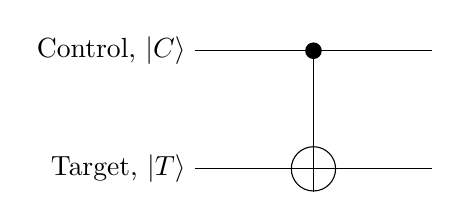
\begin{tikzpicture}
        \draw (0,0) node[anchor=east] {Target, $|T\rangle$} -- (3,0);
        \draw (0,1.5) node[anchor=east] {Control, $|C\rangle$} -- (3,1.5);
        \fill (1.5,1.5) circle (3pt);
        \draw (1.5,0) circle (8pt);
        \draw (1.5,1.5) -- (1.5,-0.3);
    \end{tikzpicture}
\end{figure}
What does it do?
If C is in state $|1\rangle$, then NOT on T, otherwise we do nothing. 
This can be written as a matrix:
\begin{align}
    \text{CNOT} &= \begin{pmatrix} 1 & 0 & 0 & 0 \\ 0 & 0 & 0 & 0 \\ 0 & 1 & 0 & 0 \\ 0 & 0 & 0 & 1 \\ 0 & 0 & 1 & 0 \end{pmatrix} \approx \begin{Bmatrix} |00\rangle \\ |01\rangle \\ |10\rangle \\ |11\rangle\end{Bmatrix},
\end{align}
where the final term is in roughly what each line represents in the $4\times4$ matrix. 
For the first two lines, where A is in $|0\rangle$, we do nothing to B, hence the identity form; the latter two lines, where A is in $|1\rangle$, we perform NOT on B - this resembles the Pauli $\hat{\sigma}_x$ matrix. 
This is also called the Controlled-X (CX) gate, where X represents that Pauli $\hat{\sigma}_x$ matrix. 
\begin{figure}[H]
    \centering
    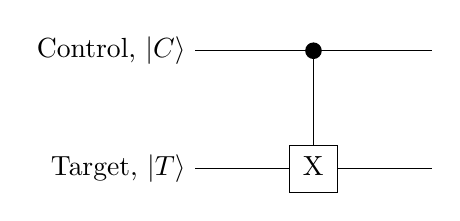
\begin{tikzpicture}
        \draw (0,0) node[anchor=east] {Target, $|T\rangle$} -- (1.2,0);
        \draw (1.8,0) -- (3,0);
        \draw (0,1.5) node[anchor=east] {Control, $|C\rangle$} -- (3,1.5);
        \fill (1.5,1.5) circle (3pt);
        \draw (1.5,1.5) -- (1.5,0.3);
        \draw (1.2,-0.3) rectangle (1.8,0.3) node[anchor=north,xshift=-8.6pt,yshift=-0.5pt] {X};
    \end{tikzpicture}
\end{figure}
CNOT clearly involves entanglement then. 
We cannot separate CNOT into a product of single-qubit matrices, e.g.
\begin{align}
    \text{CNOT} &\neq \hat{\sigma}_0\otimes\hat{\sigma}_x.
\end{align}
So CNOT is an entangling operator. 

\begin{example}[CNOT creates entanglement]
    Our Control and Target inputs are:
    \begin{figure}[H]
    \begin{multicols}{2}
        \begin{center}
        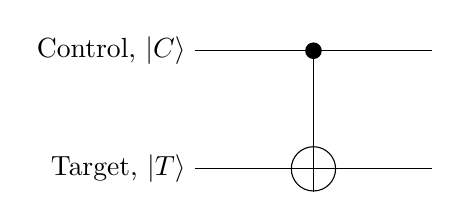
\begin{tikzpicture}
            \draw (0,0) node[anchor=east] {Target, $|T\rangle$} -- (3,0);
            \draw (0,1.5) node[anchor=east] {Control, $|C\rangle$} -- (3,1.5);
            \fill (1.5,1.5) circle (3pt);
            \draw (1.5,0) circle (8pt);
            \draw (1.5,1.5) -- (1.5,-0.3);
        \end{tikzpicture}
        \end{center}
    \columnbreak
    \begin{align}
        |C\rangle &= |+\rangle = \frac{1}{\sqrt{2}}\left(|0\rangle+|1\rangle\right) \\
        |T\rangle &= |0\rangle.
    \end{align}
    \end{multicols}
    \end{figure}
    \vspace{-2em}
    The full input state is then
    \begin{align}
        |C\rangle\otimes|T\rangle &= \frac{1}{\sqrt{2}}\left(|0\rangle+|1\rangle\right)\otimes|0\rangle \\
                       |CT\rangle &= \frac{1}{\sqrt{2}}\left(|00\rangle+|10\rangle\right).
    \end{align}
    This is a \textbf{product state} - there is no entanglement between these yet. 
    Now we pass this product state through the CNOT operator to give
    \begin{align}
        \text{CNOT}|CT\rangle &= \frac{1}{\sqrt{2}}\left(|00\rangle+|11\rangle\right),
    \end{align}
    where we not have the Bell state which is maximally entangled by definition. 
    Therefore, we see \textit{CNOT creates entanglement.}

    Let's work through this again in matrix form.
    \begin{align}
        |CT\rangle &= \frac{1}{\sqrt{2}}\begin{pmatrix} 1 \\ 1\end{pmatrix}\otimes\begin{pmatrix}1\\0\end{pmatrix} = \frac{1}{\sqrt{2}}\begin{pmatrix} 1\\0\\1\\0\end{pmatrix}. \\
        \text{CNOT}|CT\rangle &= \begin{pmatrix} 1 & 0 & 0 & 0 \\ 0 & 0 & 0 & 0 \\ 0 & 1 & 0 & 0 \\ 0 & 0 & 0 & 1 \\ 0 & 0 & 1 & 0 \end{pmatrix}\frac{1}{\sqrt{2}}\begin{pmatrix}1\\0\\1\\0\end{pmatrix}\\
                              &= \frac{1}{\sqrt{2}}\begin{pmatrix}1\\0\\0\\1\end{pmatrix} \approx \begin{Bmatrix} |00\rangle \\ |01\rangle \\ |10\rangle \\ |11\rangle\end{Bmatrix} \\
                              &= \frac{1}{\sqrt{2}}\left(|00\rangle+|11\rangle\right) = |\Phi^+\rangle.
    \end{align}
    We get the same result as before. 
\end{example}

\subsection{How to realise CNOT?}
We consider a conditional Ramsey interferometer:
\begin{figure}[H]
    \centering
    \begin{tikzpicture}
        %Nodes
        \node[squarenode] (maintopic) {H};
        \node (uppercircle) [above right=2em and 7em of maintopic] {};
        \node[squarenode] (lowercircle) [below right=2em and 7em of maintopic] {$-1$};
        \node[squarenode] (output) [right=15em of maintopic] {H};
        \node (start) [left=1em of maintopic] {$|T\rangle$};
        \node (end) [right=1em of output] {};
        \node (ups) [above right=0.7em and 3.7em of maintopic] {};
        \node (ds) [below right=0.9em and 3.1em of maintopic] {};
        \node (upe) [above left=0.7em and 3.9em of output] {};
        \node (de) [below left=0.9em and 3em of output] {};

        \node (start2) [below=4.7em of start] {$|C\rangle$};
        \node (end2) [below=5.7em of end] {};
        \node[squaredash] (main2) [below=5em of maintopic] {$\cdots$};
        \node[squaredash] (out2) [below=5em of output] {$\cdots$};
        \node (u2) [above right=0.7em and 3.5em of main2] {};
        \node (l2) [below right=0.7em and 3.7em of main2] {};
        \node (u2e) [above left=0.7em and 3.3em of out2] {};
        \node (l2e) [below left=0.7em and 3.7em of out2] {};
        \node (down2) [below right=2em and 7em of main2] {};
        \node (zero0) [above right=0.3em and 0.3em of maintopic] {$|0\rangle$};
        \node (one1) [below right=0.3em and 0.3em of maintopic] {$|1\rangle$};
        \node (one2) [above right=0.3em and 0.3em of main2] {$|1\rangle$};
        \node (zero1) [below right=0.3em and 0.3em of main2] {$|0\rangle$};

        %Lines
        \draw (start.east) -- (maintopic.west);
        \draw (output.east) -- (end.west);
        \draw (maintopic.east) cos (ups) sin (uppercircle);
        \draw (maintopic.east) cos (ds) sin (lowercircle.west);
        \draw (uppercircle) cos (upe) sin (output.west);
        \draw (lowercircle.east) cos (de) sin (output.west);
        \draw (start2.east) -- (main2.west);
        \draw (out2.east) -- (end2.west);
        \draw (main2.east) cos (u2) sin (lowercircle.west);
        \draw (lowercircle.east) cos (u2e) sin (out2.west);
        \draw (main2.east) cos (l2) sin (down2);
        \draw (down2) cos (l2e) sin (out2.west);
    \end{tikzpicture}
\end{figure}

If the Control is in state $|1\rangle$, then it applies a $-1$ factor to the state vector and this $-1$ factor flips the output of the Ramsey interferometer, i.e. perform the NOT.

\section{Implementing Quantum Computing in real physical systems}
We have a choice of our five possiblities:
\begin{enumerate}
    \item Atoms
    \item Ions 
    \item Semiconductors
    \item Superconductors
    \item Photons
\end{enumerate}
We are going to use atoms from here, but the question is how to satisfy the 5 diVincenzo criteria:
\begin{enumerate}
    \item Initialisation: prepare qubits
    \item Gates: single-qubit rotations and two-qubit gates (CNOT)
    \item Read-out.
    \item Low decoherence.
    \item Scalability.
\end{enumerate}

\chapter{Rydberg Atom Quantum Computer}
\begin{enumerate}
    \item Preparation: laser cooling (Nobel Prize 1997), and trapping with optical tweezers (Nobel Prize 2018) are used to assemble the atoms into our qubit states, all into state $|0\rangle$ for example to begin with.
    \item Gates: qubit gates created using Rydberg states and dipole-dipole interactions.
\end{enumerate}

\textbf{Strike Impacts:}
\begin{itemize}
    \item Thursday Week 16 and possibly workshop Week 16
    \item Tuesday Week 17 and possibly workshop Week 17
    \item All lectures Week 18 and 19
\end{itemize}
These are the possible impacts of striking, if Charles strikes. 
We need to believe in the many worlds interpretation of quantum mechanics and only by coming to the lectures and collapsing the wavefunction will we find out if we are in a universe where he is striking or not.
The question of what universe Charles is in has been one considered by some of the greatest thinkers of modern times; the results are inconclusive. 

\section{Optical Tweezing}
We use one focussed laser beam to move an atom and place it exactly where we want it.
Light exerts a force on atoms and they are forced either to the ends of the beam or the focus of it.
Two types of light force:
\begin{itemize}
    \item Optical dipole force - cycles of absorption (stimulated emission and trapping)
    \item Spontaneous scattering force - cycles of absorption (spontaneous emissing and cooling)
\end{itemize}   
For our optical dipole potential, we recall the two state model, with $\hbar\om_0$ between $|g\rangle$ and $|e\rangle$, leading to the detuning frequency $\Delta$.
\begin{figure}[H]
    \centering
    \begin{tikzpicture}
        \draw[-Latex] (4,1) node[anchor=north] {EM field} sin (4.5,1.5) cos (5,1) sin (5.5,0.5) cos (5.75,0.75) sin (6,1.1) cos (6.2,0.8) sin (6.35,0.6) cos (6.9,0.9);
        \draw (8,1) circle (30pt);
        \draw (7.3,0.4) node[anchor=east,xshift=-5pt] {$|g\rangle$} -- (8.7,0.4) node[anchor=north,midway,yshift=-10pt] {$\Delta<0$};
        \draw (7.3,1.6) node[anchor=east,xshift=-5pt] {$|e\rangle$} -- (8.7,1.6);
        \draw[dashed] (7.3,1.3) -- (8.7,1.3);
        \draw[Latex-Latex] (7.8,0.4) -- (7.8,1.6) node[anchor=east,midway] {$\hbar\om_0$};
        \draw[-Latex,thick,red] (8.3,0.4) -- (8.3,1.3);

        \draw[dashed] (9.4,0.4) -- (10.8,0.4) node[anchor=north,midway] {$\Delta=\om-\om_0$};
        \draw[dashed] (9.4,1.3) -- (10.8,1.3) node[anchor=west,xshift=10pt] {$|g,1\rangle$};
        \draw[dashed] (9.4,1.6) -- (10.8,1.6) node[anchor=west,xshift=10pt] {$|e,0\rangle$};
        \draw[-Latex] (10.5,2) -- (10.5,1.6);
        \draw[-Latex] (10.5,0.9) -- (10.5,1.3) node[anchor=west,midway] {$\hbar\om$};
    \end{tikzpicture}
\end{figure}
We can form our interaction operator as we have done previously when looking at the Rabi model, yielding
\begin{align}
    \Ham_{int} &= \frac{\hbar}{2}\begin{pmatrix}\Delta & \Omega \\ \Omega & -\Delta\end{pmatrix}.
\end{align}
We do not consider between $|g\rangle$ and $|e\rangle$, but $|g,1\rangle$ (the ground state plus a photon) and $|e,0\rangle$ (the excited state with no photon).
These states are only slightly separated by $\hbar(\om_0-\om)$, i.e. $-\hbar\Delta$, from which we can see we have chosen negative detuning where $\Delta < 0$.
This gives our bare states when $\Omega=0$, and then we see that increasing $\Omega$ \emph{dresses} the states, increasing the upper state and decreasing the lower state.
\begin{align}
    \Ham_{int} &= \frac{\hbar}{2}\begin{pmatrix}\Delta & \Omega \\ \Omega & -\Delta\end{pmatrix}.
\end{align}
The energies of the states in the laser field are given by the eigenvalues of $\Ham_{int}$:
\begin{align}
    \left(\Ham_{int}-\frac{\hbar}{2}\lambda\hat{\sigma}_0\right)\begin{pmatrix}a\\ b\end{pmatrix} &= 0 \\
    \frac{\hbar}{2}\begin{vmatrix} \Delta-\lambda & \Omega \\ \Omega & -\Delta-\lambda \end{vmatrix} &= 0 \\
    -\Delta^2+\lambda^2-\Omega^2 &= 0 
\end{align}
\begin{align}
    \lambda^2 &= \Delta^2+\Omega^2 \\
    \lambda &= \pm\sqrt{\Delta^2+\Omega^2} \\
    E_{\pm} &= \pm\frac{\hbar}{2}\sqrt{\Delta^2+\Omega^2},
\end{align}
where $E_\pm$ are our eigenenergies.
We choose $\Delta<0$ (red detuning), and $|\Delta|\gg\omega$ (far detuned to avoid spontaneous emission).
We then get
\begin{multicols}{2}
\begin{figure}[H]
    \centering
    \begin{tikzpicture}
        \draw (0,0) node[anchor=east] {$-\hbar\frac{\Delta}{2}$} -- (2,0) node[anchor=north,midway] {$|g,1\rangle$} -- (3,-0.5) -- (5,-0.5);
        \draw (0,1.5) node[anchor=east] {$+\hbar\frac{\Delta}{2}$} -- (2,1.5) node[anchor=south,midway] {$|e,0\rangle$} node[anchor=south,midway,yshift=15pt] {\shortstack{$\Omega = 0$ \\ Bare States}} -- (3,2) -- (5,2) node[anchor=south,midway] {\shortstack{$\Omega>0$ \\ Dressed States}};
        \draw[dashed] (3,0) -- (5,0);
        \draw[Latex-Latex] (4.7,-0.5) -- (4.7,0) node[anchor=west,midway] {$U_0 = -\frac{\hbar\Omega^2}{4|\Delta|}$};
    \end{tikzpicture}
\end{figure}
\columnbreak
\begin{align}
    E_\pm &= \pm\frac{\hbar}{2}|\Delta|\sqrt{1+\frac{\Omega^2}{|\Delta|^2}} \\
          &= \pm\frac{\hbar}{2}|\Delta|\left(1+\frac12\frac{\Omega^2}{|\Delta|^2}\right) \\
          &= \pm\frac{\hbar}{2}|\Delta|\pm \frac{\hbar\Omega^2}{4|\Delta|}.
\end{align}
\end{multicols}
The shift of the lower state, 
\begin{align}
    U_0 &= -\frac{\hbar\Omega^2}{4|\Delta|},
\end{align}
is known as the \textbf{Light Shift} (or ac-Stark shift).
This tells use the depth of the optical tweezer indent(handwriting?). 
We want to rewrite this in terms of laser intensity. 
Recall that
\begin{align}
    \Omega &= -\frac{d\mathcal{E}}{\hbar}, & I &= \frac12 c\e_0\mathcal{E}^2.
\end{align}
The dipole moment $d$ is related to the spontaneous emission rate of the excited state $|e\rangle$, $\Gamma$, by
\begin{align}
    \Gamma &= \frac{d^2}{3\pi\e_0(\lambda_0/2\pi)^3},
\end{align}
where $\lambda_0$ is the wavelength of the transition $|g\rangle\to|e\rangle$, $\om_0=\frac{2\pi c}{\lambda_0}$.
Using these, 
\begin{align}
    \Omega &= \Gamma\sqrt{\frac{I}{2I_s}}, \text{ where } I_s = \frac{\pi}{3}\frac{hc\Gamma}{\lambda_0^3}
\end{align}
is the saturation intensity. 
Our optical tweezer trap depth is now
\begin{align}
    U_0 &= -\frac{\hbar\Omega^2}{4|\Delta|} = -\frac{\hbar\Gamma^2}{4|\Delta|}\frac{I}{2I_s}.
\end{align}
The trap depth $U_0$ is proportional to the laser intensity and inversely proportional to detuning, $|\Delta|$.
We set the limit of large detuning to avoid spontaneous emission, but this impacts the trap depth. 
To get this back, however, we use a large laser intensity. \\
A laser beam is described by
\begin{align}
    I(x,y,z) &= I_0\frac{w_0^2}{w^2}e^{-2(x^2+y^2)/w^2}, & w &= w_0\left(1+\frac{z^2}{z_R^2}\right)^{1/2}, & z_R &= \frac{\pi w_0^2}{\lambda}.
\end{align}
We can therefore plot what the potential $U_0$ looks like as $U_0(x,y,z)$:
\begin{figure}[H]
    \centering
    \begin{tikzpicture}
        \draw[-Latex] (-4,0) -- (4,0) node[anchor=north] {$z$};
        \draw[-Latex] (0,-2) -- (0,2) node[anchor=east] {$U_0$};
        \draw (-4,1.8) sin (0,0.3) cos (4,1.8);
        \draw (-4,-1.8) sin (0,-0.3) cos (4,-1.8);
        \draw[ultra thick] (-0.1,0.25) -- (0.1,0.25) node[anchor=south,xshift=5pt] {$w_0$};

        \draw[-Latex] (-4.5,-2) -- (-4.5,2);
        \draw[-Latex] (-6,0) node[anchor=east] {$U_0$} -- (-4.2,0);
        \draw (-5.8,0) .. controls (-5.8,1) and (-4.4,0.2) .. (-4.5,2);
        \draw (-5.8,0) .. controls (-5.8,-1) and (-4.4,-0.2) .. (-4.5,-2);

        \draw[-Latex] (0,-4.3) -- (0,-2.7);
        \draw[-Latex] (-4,-3) -- (4,-3);
        \draw (-4,-3) cos (-2,-3.5) sin (0,-4) cos (2,-3.5) sin (4,-3);
        \draw (-0.1,-4) -- (0.1,-4) node[anchor=west,yshift=-5pt] {$-U_0$};
    \end{tikzpicture}
\end{figure}
The atom is now trapped at the focus in all 3 dimensions, giving us an optical tweezer.
Consider
\begin{align}
    \ifnt I(z=0)\,dx\,dy &= P \implies I_0 = \frac{2P}{\pi w_0^2},
\end{align}
where $P$ is the laser power. 
This tells us that we want to have as powerful a laser as possible, with a smaller beam waist size. 
However, we cannot focus the beam waist arbitrarily small because diffraction and other effects will take hold. 
Typically, $w_{0,min}\approx \lambda$.

\chapter{}

\begin{example}[Workshop 2, Question 2: Ramsey Interferometry and Decoherence]
    The Hadamard is how we read out the `phase' of the state vector. 
    Why is that?
    We take a general state (as in part c of question),
    \begin{align}
        |\psi\rangle &= \begin{pmatrix} ae^{-i\Delta t/2} \\ be^{i\Delta t/2} \end{pmatrix}.
    \end{align}
    Then we must take the density matrix for this state - where it is a pure state, so it is completely coherent and has a well-defined state.
    To describe decoherence, which is due to interaction with the environment, we use the density matrix description because it allows for mixed states, i.e. states without perfectly defined phases.
    \begin{align}
        \rho &= |\psi\rangle\langle\psi| = \begin{pmatrix} |a|^2 & ab^*e^{-i\Delta t} \\ ba^*e^{i\Delta t} & |b|^2 \end{pmatrix},
    \end{align}
    where the diagonal terms represent the probability to be in each state, and the off-diagonal terms are called \textbf{Coherences} which contain all the information about phase.\\
    These may contain all the \emph{wave} information, but not necessarily all the \emph{quantum} information. 
    If a state decoheres completely, i.e. coherence decay to zero:
    \begin{align}
        \rho_{dec} &= \begin{pmatrix} |a|^2 & 0 \\ 0 & |b|^2\end{pmatrix}\\
                   &= |a|^2|0\rangle\langle0| + b^2|1\rangle\langle1|,
    \end{align}
    so we still have a superposition, but no phase information. 
    This is called a \textbf{mixed state.}

    For the read-out process, we go back to earlier on in the question now. 
    We define a general density matrix as
    \begin{align}
        \rho &=  \frac12\begin{pmatrix} 1+w & u-iv \\ u+iv & 1-w\end{pmatrix}.
    \end{align}
    We now use the Hadamard to modify the density matrix, yielding
    \begin{align}
        \rho'= \hat{H}\rho\hat{H}^\dagger &= \frac12\begin{pmatrix} 1+u & w+iv \\ w-iv & 1-u\end{pmatrix}.
    \end{align}
    The probability to be in $|0\rangle$ is then
    \begin{align}
        P_{|0\rangle} &= \frac12(1+u),
    \end{align}
    where we can now read out the real part of coherence.
    The Hadamard is used to measure the coherence of the qubit, by projecting the real part of the coherence $u$ from the off-diagonals to the diagonals.

    Now let's jump down to part f of the question because Charles says so. 
    We transform $u\to ue^{-it/T_2}$, where $T_2$ is some time constant representing how the coherence decays.
    The probability will be modified by this, showing a decaying and oscillating amplitude:
    \begin{align}
        P_{|0\rangle} &= \frac12(1+ue^{-t/T_2}),\quad u=\cos(\Delta t) \\
                      &= \frac12(1+\cos(\Delta t)e^{-t/T_2}).
    \end{align}
    \begin{figure}[H]
        \centering
        \begin{tikzpicture}
            \draw[-Latex] (-2,0) -- (6,0) node[anchor=north] {$\Delta$};
            \draw[-Latex] (2,0) -- (2,2.8) node[anchor=south] {$P_{|0\rangle}$};
            \draw[purple] (-2,0) cos (-1,1.25) sin (0,2.5) cos (1,1.25) sin (2,0) cos (3,1.25) sin (4,2.5) cos (5,1.25) sin (6,0);
            \draw[cyan,dashed] (-2,2.5) cos (-1,1.25) sin (0,0) cos (1,1.25) sin (2,2.5) node[anchor=north east,black] {1} cos (3,1.25) sin (4,0) cos (5,1.25) sin (6,2.5);
        \end{tikzpicture}
    \end{figure}
    These are the Ramsey fringes for $t\ll T_2$. 
    Pure states are good because we have no decoherence, so quantum computing will work. 
    Over time, the oscillations can get smaller, begin to vibrate around $\frac12$, so the Ramsey fringe visibility is reduced, leading to decoherence.
    Working at low temperatures, i.e. mK, reduces likelihood of decoherence.
\end{example}

\section{Optical Tweezing Ctd.}
We used a laser to trap an atom qubit in its beam, with
\begin{align}
    U_0 &= -\frac{\hbar\Omega}{4|\Delta|}, & \Omega &= \Gamma\sqrt{\frac{I}{2I_s}}.
\end{align} 
The trap depth is proportional to the laser intensity (and power):
\begin{align}
    I &= I_0\frac{w_0^2}{w^2}e^{-2(x^2+y^2)/w_0^2}.
\end{align}
\emph{doodle}
The trap depth forms a harmonic potential, $\frac12 m\om_zz^2$.
This means we want to cool the atom to its Harmonic Oscillator ground state.
\emph{doodle}
This is the minimum size of the atomic wave packet.
We then send in our laser beam with an electric field,
\begin{align}
    \mathcal{E} &= \mathcal{E}_0\cos(\phi_L-\om t),\quad \phi_L = \vec{k}\cdot\vr.
\end{align}
There is now an error in the phase, 
\begin{align}
    \Delta\phi_L &= k\Delta x,
\end{align}
if the field propagates in the $x$-direction (switch out $x$ for $y$ or $z$ depending on propagation direction).
This error is a source of decoherence, so we need to try and minimise it. 
However, the scaling is very bad, on the order of needing $10^4$ more laser power to decrease $\Delta x$ by a factor of 10.
\begin{figure}[H]
    \centering
    \begin{tikzpicture}
        \draw (0,0) node[anchor=east] {$|g\rangle$} -- (1.5,0);
        \draw[dashed] (0,1.3) -- (1.5,1.3);
        \draw (0,1.6) node[anchor=east] {$|e\rangle$} -- (1.5,1.6);
        \draw[-Latex] (0.3,0) -- (0.3,1.6) node[anchor=east,midway] {$\hbar\om_0$};
        \draw[-Latex,red,thick] (1.2,0) -- (1.2,1.3) node[anchor=east,midway] {$\hbar\om$};
        \draw[snake it,-Latex,red] (1.4,1.6) -- (1.6,0.8);
    \end{tikzpicture}
\end{figure}
\vspace{-20pt}
\begin{align}
    \Delta &= \om-\om_0 < 0, \\
    |\Delta| &\gg \Omega.
\end{align}
We need $|\Delta|$ large to avoid the decay of our excited state $|e\rangle$.
Calculating the probability that qubit scatters a photon, we have
\begin{itemize}
    \item spontaneous decay rate of $|e\rangle$ is $\Gamma$
    \item the photon scattering rate is $R=\Gamma P_{|e\rangle}$
    \item $P_{|e\rangle}$ is the probability to be in state $|e\rangle$; for a two-level model, this is $|b|^2$
\end{itemize}
This model, however, did not include the possiblity of decay, so we need to add decay to our equations of motion of the Bloch vector.
From Workshop 1,
\begin{align}
    \begin{pmatrix} \dot u \\ \dot v \\ \dot w \end{pmatrix} &= \begin{pmatrix} 0 &-\Delta &0\\ \Delta & 0 & -\Omega \\ 0 & \Omega & 0 \end{pmatrix}\begin{pmatrix}u \\ v \\ w\end{pmatrix}.
\end{align}
Where the RHS is Torque$\times$Bloch vector. 
We now have
\begin{align}
    \dot{u} &= -\frac{u}{T_2} - \Delta v, \\
    \dot{v} &= \Delta u - \frac{v}{T_2} - \Omega w, \\
    \dot{w} &= \Omega v - \frac{1}{T_1}(w-1).
\end{align}
$T_2$ is the decay of coherence; $T_1$ is the decay of population. 
These are the \textbf{Optical Bloch Equations.}

\chapter{Spontaneous Photon Scattering}
In our optical tweezer model described above, not all photons going into the qubit will hit the same way, so sometimes we will have scattering of photons off the photon. 
Last time we discussed spontaneous emission from the excited state, $\Gamma$, where the rate of spontaneous scattering can then be described as
\begin{align}
    R &= \Gamma P_{|e\rangle}.
\end{align}

\section{Optical Bloch Equations}
If spontaneous emission is the only decoherence/decay mechanism, then
\begin{align}
    T_1 &= \frac{1}{\Gamma}, & T_2 &= \frac2\Gamma, \\ 
    \frac{1}{T_1} &= \Gamma = \frac1\tau, & \frac1{T_2} &= \frac{\Gamma}{2}, 
\end{align}
where $\tau$ is the lifetime of the excited state.
We can then substitute these into the optical Bloch equations defined last lecture, yielding
\begin{align}
    \dot{u} &= -\frac{\Gamma}{2}u - \Delta v, \\
    \dot{v} &= \Delta u - \frac{\Gamma}{2}v - \Omega w, \\
    \dot{w} &= \Omega v - \Gamma(w-1).
\end{align}
From here, we solve for the steady state, $\dot u = \dot v = \dot w = 0.$
Following lots of algebra, we find
\begin{align}
    P_{|e\rangle} &= \frac12\left(1-w_{ss}\right) = \frac{\Omega^2/4}{\Delta^2 + \Gamma^2/4 + \Omega^2/2}.
\end{align}
\textbf{This is one of our Very Important Equations.}
We want to plot this for three cases:
\begin{enumerate}
    \item Small $\Omega$: $\Omega\ll|\Delta|$ and $\Gamma$. (NB: not the case for optical tweezer!) 
        \begin{align}
            P_{|e\rangle} &\approx \frac{\Omega^2/4}{\Delta^2 + \Gamma^2/4}.
        \end{align}
        This corresponds to weak driving, where it will result in low intensity and low probability.
        This equation will look familiar as a Lorentzian, or a Cauchy distribution. 
        \emph{doodle}
        \begin{figure}[H]
            \centering
            \begin{tikzpicture}
                \draw (-4,0) -- (4,0);
                \draw (0,0) -- (0,3);
                \draw (-4,0.1) .. controls (-1.2,0) and (-0.5,3) .. (0,2.7);
                \draw (0,2.7) .. controls (0.5,3) and (1.2,0) .. (4,0.1);
            \end{tikzpicture}
        \end{figure}
        Our Full Width Half Maximum is then
        \begin{align}
            \text{FWHM} &= \Gamma = \frac{1}{T_1}=\frac{1}{\tau},
        \end{align}
        which is the natural width of $|g\rangle\to|e\rangle$ transition.
    \item $\Delta=0$, i.e. on resonance. 
        Again, not like our tweezer where we are very far from resonance. 
        Now, we have a probability of
        \begin{align}
            R_{|e\rangle} &= \frac{\Omega^2/4}{\Gamma^2/4 + \Omega^2/2}.
        \end{align}
        We can then plot the probability, now against $\Omega^2$:
        \begin{figure}[H]
            \centering
            \begin{tikzpicture}
                \draw (0,0) -- (4,0);
                \draw (0,0) -- (0,3);
                \draw (0,0) .. controls (1.3,1.4) .. (4,1.5);
                \draw[dashed] (0,1.5) -- (4,1.5);
            \end{tikzpicture}
        \end{figure}
        \begin{align}
            \frac{\Omega^2}{2} &= \frac{\Gamma^2}{4} \implies P_{|e\rangle} = 0.25
        \end{align}
        This is linear for $\Omega<\Gamma$.
        Then
        \begin{align}
            \Omega^2 &= \Gamma^2\frac{I}{2I_S}, & P_{|e\rangle} &= 0.25 \text{ for } I=I_S,
        \end{align}
        where $I_S$ is the saturation intensity. 
    \item $|\Delta|\gg\Gamma,\Omega$, i.e. the case for optical tweezing.
        $\Omega\gg\Gamma$ also.
        We have strong driving and strong detuning.
        \begin{align}
            P_{|e\rangle} &= \frac{\Omega^2/4}{\Delta^2} = \frac{\Omega^2}{4\Delta^2}.
        \end{align}
        Therefore, the photon scattering rate in an optical tweezer is
        \begin{align}
            R &= \Gamma P_{|e\rangle} = \Gamma\frac{\Omega^2}{4\Delta^2}.
        \end{align}
        Now to the trap depth, 
        \begin{align}
            U_0 &= -\frac{\hbar\Omega^2}{4|\Delta|} \implies \frac{|U_0|}{R} &= \frac{\hbar\Omega^2/4|\Delta|}{\Gamma\Omega^2/4\Delta^2} = \hbar\left(\frac{\Delta}{\Gamma}\right).
        \end{align}
        So we want to use $\Delta\gg\Gamma$ to minimise scattering for a given trap depth, i.e. \emph{far detuning.}
\end{enumerate}
We can use spontaneous scattering for cooling!
Laser cooling works through a spontaneous scattering force.
Each scattering event cause a recoil on the qubit or atom.
\emph{doodle}
Cycles of excitation and decay transfer, on average, $\hbar\vec{k}$ of momentum to the atom per cycle.
This exerts a force
\begin{align}
    \vec{F} &= \hbar\vec{k}R = \hbar\vec{k}\Gamma P_{|e\rangle} \\
            &= \hbar\vec{k}\Gamma\frac{\Omega^2/4}{\Delta^2+\Gamma^2/4+\Omega^2/2}.
\end{align}
This force is called the \textbf{Spontaneous Scattering Force.}
The properties of this force will then follow the previous discussions on the behaviour of the probability in different regimes.

How will we use this force for cooling?
Use 2 counter-propagating lasers, both red detuned. 
\emph{doodle}
The force on the atom is then the sum of the force from laser 1 and laser 2:
\begin{align}
    F &= F_+ + F_-.
\end{align}
If the atom is moving, however, there is a Doppler shift. 
\begin{itemize}
    \item Laser 1: it's moving away, so detuning, $\Delta\to\Delta-kv_{atom}$.
    \item Laser 2: it's moving towards, so detuning, $\Delta\to\Delta+kv_{atom}$.
\end{itemize}
\begin{align}
    F_{\pm} &= \pm \hbar\vec{k}\Gamma\frac{\Omega^2/4}{\Gamma^2/4 + \Omega^2/2 + (\Delta\mp kv_{atom})^2}.
\end{align}









\end{document}


























